\section{Radds存储系统总体设计}

	
	
	\subsection{存储系统架构设计}

	Radds存储系统总体架构组成如下所示
	
	\begin{figure}[H]
		\centering
		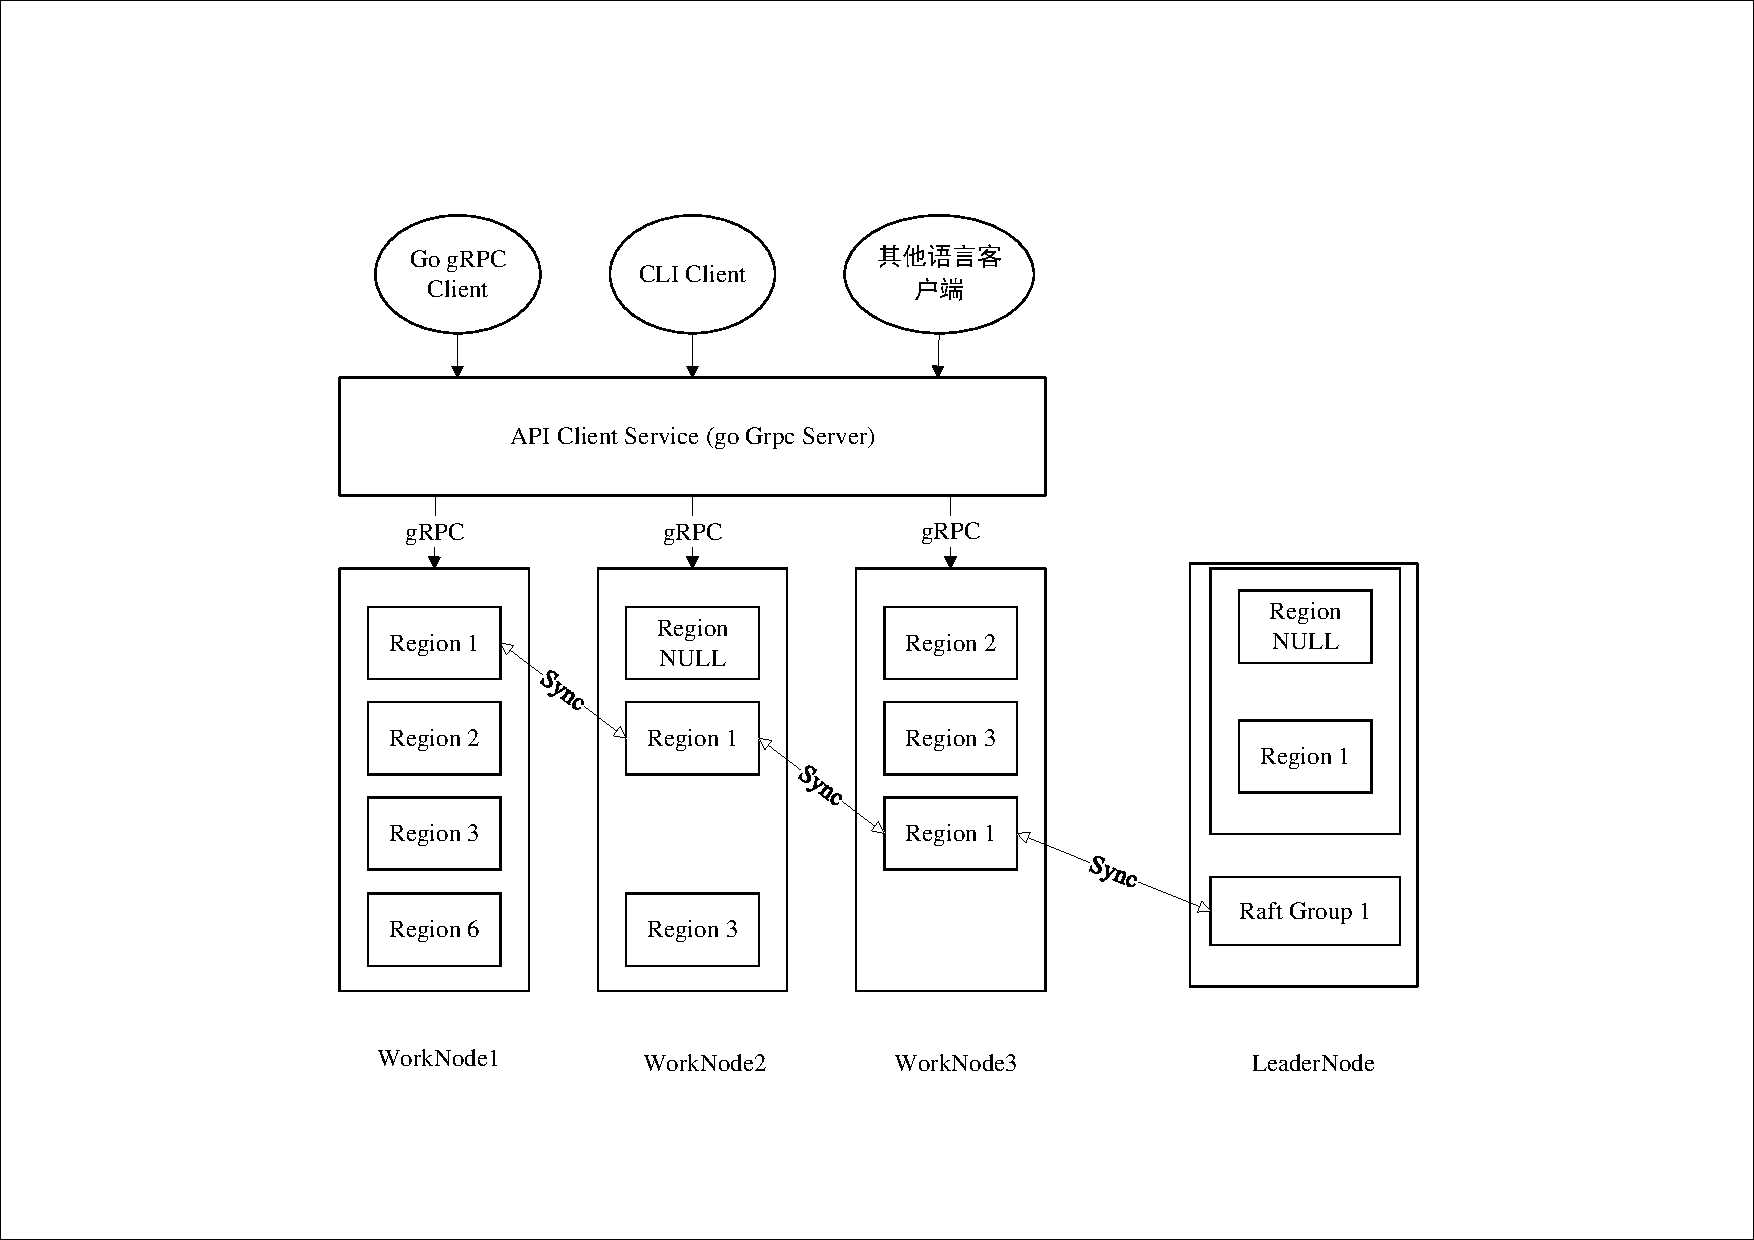
\includegraphics[width=0.80\textwidth]{pdf/radds_system_arch.pdf}
		\caption{Radds存储系统总体架构图}
		\label{overall_structure}
	\end{figure}

		系统的设计架构是C/S的方式,并提供最大能力的可插拔特性。服务端支持单机模式和集群模式;客户端提供了API Client中台,
		默认使用gRPC通信,客户端支持多语言:默认支持golang语言的gRPC客户端,RESTful形式的HTTP通信,还有命令行CLI方式,
		用户可以使用支持gRPC的其它语言来开发自定义的客户端(gRPC支持绝大多数主流开发语言)。
		
		\begin{enumerate}[fullwidth,itemindent=2em,listparindent=2em]
			\item 服务端 API Client中台
			
			API Client中台提供诸多功能,如:API客户端调用日志,API限流,数据查询日志,存储消息重定向等。

			\item 服务端单机模式
			
			单机模式单机模式提供键值形式的数据存储,实现了LSM-Tree结构的存储引擎,单机模式可以看做是集群模式的一个存储节点,
			
			\item 服务端集群模式
			
			集群模式以Raft算法为设计核心,集群间的节点通信使用gRPC协议的message,这种方式通信的开销更小,因为gRPC仅仅建立在TCP协议之上。
			当然一个WorkNode不是只存储一个Group的数据,还可以存储其它Group的数据。
			集群的Leader通过数据规模和API调用次数分配工作节点数量,这个Leader仅仅是一个Group的Leader,整个集群可以有多个Leader,它们分别属于不同的Group。
			集群中的一个节点如果作为一个Group的Leader,那么它存储这个Group的所有数据:用户数据,元数据,缓存数据。
			集群中的一个节点如果作为一个Group的WorkNode,那么它只存储这个Group的用户数据。
			
			集群中的一个节点会存在不同的状态,可能的情况有:
	
			(1)Leader宕机,一个Group的Leader宕机后,其它节点在超时时间内未收到心跳信息则会感知到Group Leader宕机,
			根据Raft算法选择Group的新一任Leader,当新一任的Leader选举后会向客户端中台发送消息并从客户端中台取得必要的元数据。
			
			(2)WorkNode宕机,一个Group的WorkNode宕机后,Group的Leader会在长时间未收到心跳后将此节点移除Group并重新通知客户端中台机器数量,
			以便于其它Group能分配到状态良好的机器。
			
			(3)节点存储空间异常,当一个节点的活跃Group Region的存储空间到达95\%,由于要保证分布式系统数据的强一致,
			所以无论是Leader还是WorkNode都会停止存储新的数据,这些节点的Region只能作为WorkNode存储数据提供数据查询服务,对于写操作不在响应,
			同时它们的数据版本永久定格在此刻,当新的写操作到达时,Leader会通知客户端中台,客户端中台会重新选择集群节点,根据Raft算法选择新任Leader。
			在数据归并的过程中,如果这些节点的存储空间由于数据的归并而释放到足够存储一个Region的大小(默认一个机器磁盘容量的1/4),
			那么它可以成为一个Group的Region,根据Raft算法强一致的特性,这些数据完全被丢弃成为Region NULL,这时它就可以成为被集群选中的WorkNode。
	
			(4)节点I/O异常,一个Group的不同节点只有一个节点是Leader Node,Leader对客户端进行写响应,在客户端平台看来Leader和WorkNode没有不同,
			当一个请求到达时,客户端中台分发请求到一个机器。由于所有请求都要经过客户端中台,所以当节点I/O异常,可以考虑是机器的故障,并上报中台是不可用节点。
	
			由于Raft算法形式上比较清晰,本文根据Raft算法在机器层面做了改动,让一个节点同时可以最多容纳4个Region,这样保证Leader节点不会出现太大程度的浪费,
			同时充分利用WorkNode的存储空间存储用户数据。
			对于LSM-Tree的存储结构本文则是做全部的复现,存储引擎和数据复制,数据压缩是存储系统的工作核心。
			对于客户端中台的搭建,这是一个面向用户的组成部分,也是本文的创新,这是让一个存储引擎可用和好用的部分。
			同时客户端中台设计成了一个插件化的中心,后续也可以添加新的功能,如鉴权,资源隔离,甚至可以实现多租户方案等,这个灵感来源于阅读SnowFlake数据仓库和一些数据库报告的相关论文。
	
		\end{enumerate}
		

		  
	\subsection{存储层功能总体设计}
			
	\begin{figure}[H]
		\centering
		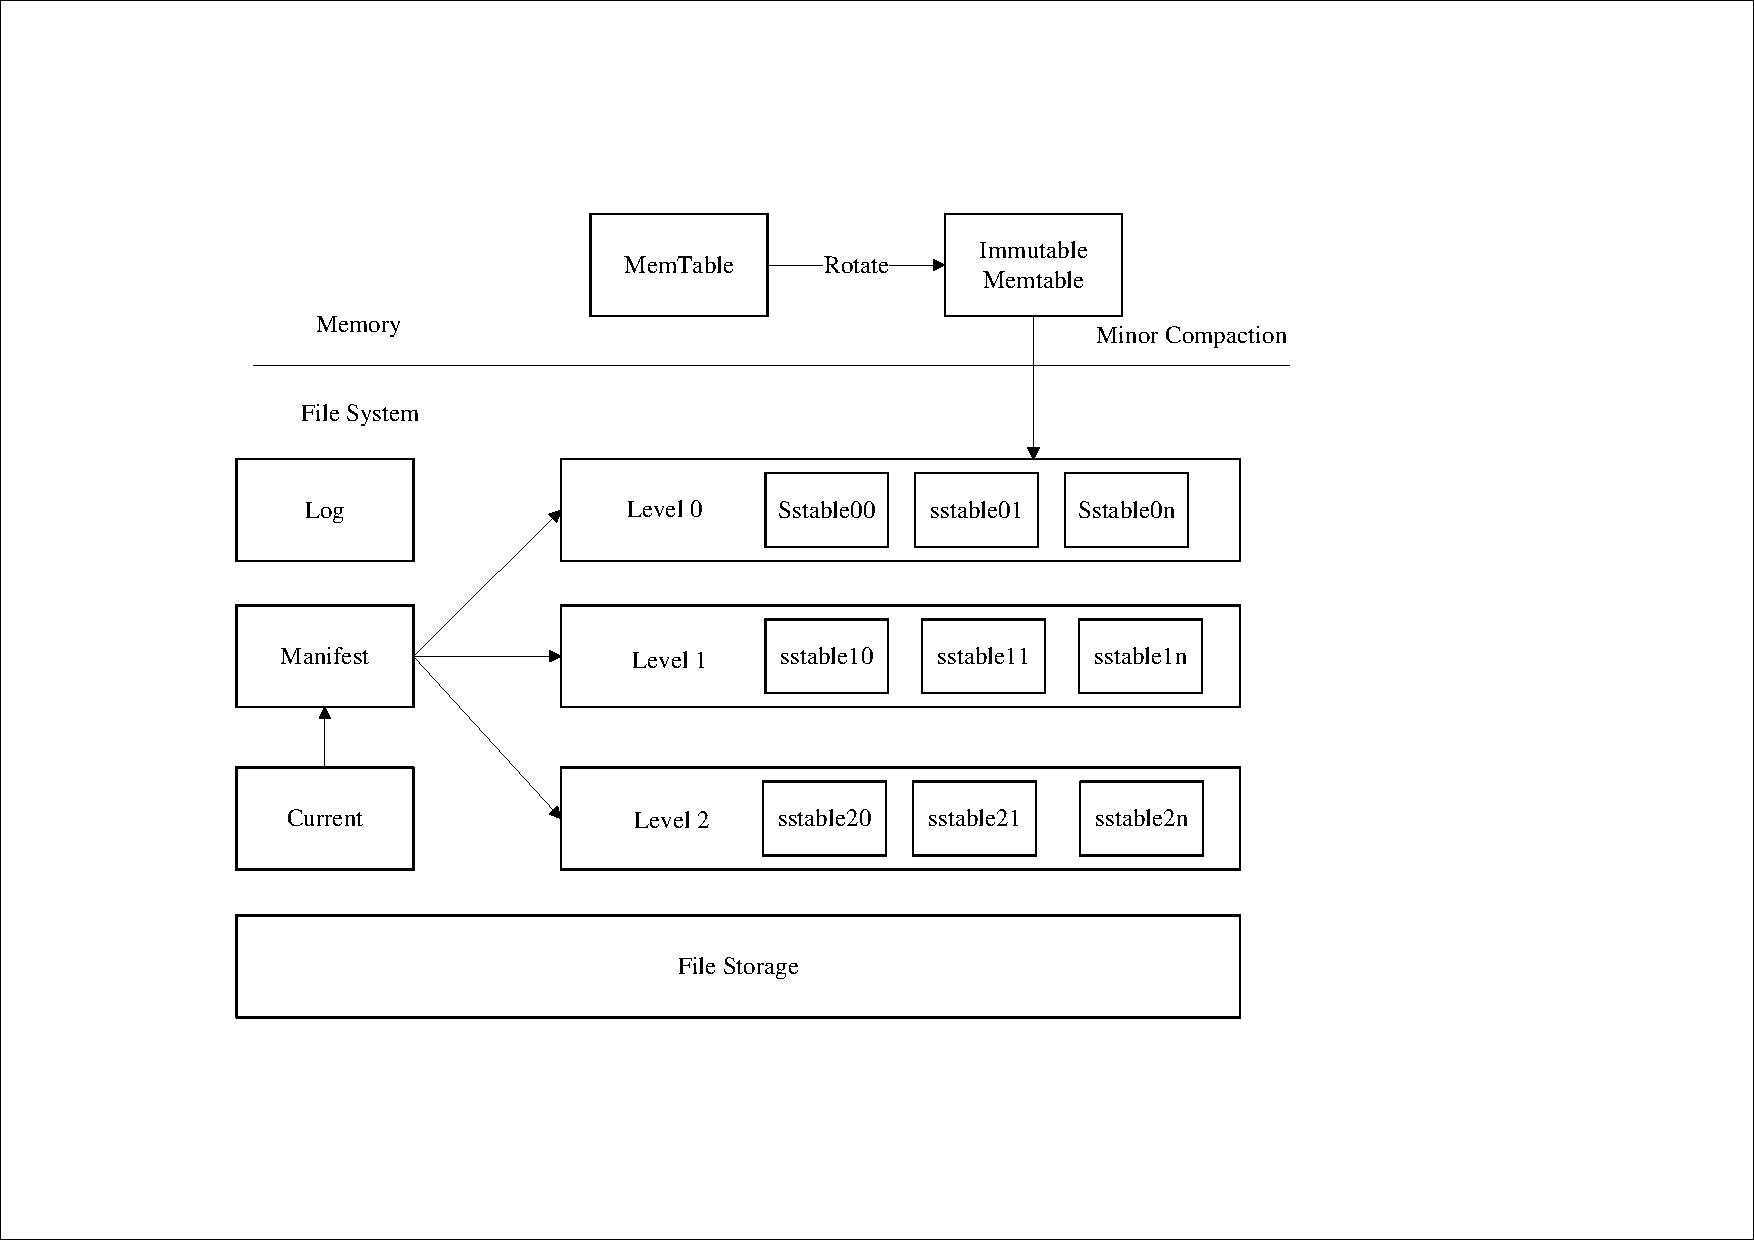
\includegraphics[width=0.95\textwidth]{pdf/leveldb_arch.pdf}
		\caption{Radds存储层架构设计}
		\label{mobile_overall_design}
	\end{figure}


		\subsubsection{存储引擎设计概述}
		
		本文要实现一个写性能优秀的存储引擎,则必须实现一个LSM树(Log Structured-Merge Tree)。LSM树的核心思想就是放弃部分读的性能,换取最大的写入能力。
		LSM树写性能极高的原理,就是尽量减少随机写的次数。对于每次写入操作,并不是直接将最新的数据驻留在磁盘中,而是将其拆分成
		
		(1){一次日志文件的顺序写}

		(2){一次内存中的数据插入}

		存储架构正是实践了这种思想,将数据首先更新在内存中,当内存中的数据达到一定的阈值,将这部分数据真正刷新到磁盘文件中,因而获得了极高的写性能(顺序写60MB/s, 随机写45MB/s)。

		\subsubsection{内存可变结构memtable总体设计}
		
		之前提到,存储引擎的一次写入操作并不是直接将数据刷新到磁盘文件,
		而是首先写入到内存中作为代替,memtable就是一个在内存中进行数据组织与维护的结构。
		memtable中,所有的数据按用户定义的排序方法排序之后按序存储,
		等到其存储内容的容量达到阈值时(默认为4MB),便将其转换成一个不可修改的memtable,
		与此同时创建一个新的memtable,供用户继续进行读写操作。
		memtable底层使用了一种跳表数据结构,这种数据结构效率可以比拟二叉查找树,
		绝大多数操作的时间复杂度为O(log n)。

		\subsubsection{内存不可变结构immutable memtable总体设计}

		memtable的容量到达阈值时,便会转换成一个不可修改的memtable,
		也称为immutable memtable。这两者的结构定义完全一样,
		区别只是immutable memtable是只读的。
		当一个immutable memtable被创建时,存储系统的后台压缩进程便会将利用其中的内容,
		创建一个sstable,持久化到磁盘文件中。

		\subsubsection{日志文件结构journal总体设计}

		存储系统的写操作并不是直接写入磁盘的,而是首先写入到内存。
		假设写入到内存的数据还未来得及持久化,存储系统进程发生了异常,抑或是宿主机器发生了宕机,
		会造成用户的写入发生丢失。因此存储系统在写内存之前会首先将所有的写操作写到日志文件中,
		也就是log文件。当以下异常情况发生时,均可以通过日志文件进行恢复:

		\begin{enumerate}
			\item 写log期间进程异常;
			\item 写log完成,写内存未完成;
			\item write动作完成(即log、内存写入都完成)后,进程异常;
			\item immutable memtable持久化过程中进程异常;
			\item 其它压缩异常(较为复杂,首先不在这里介绍);
		\end{enumerate}
	
	异常发生时,处理的情况分两种:
		\begin{enumerate}
			\item 当第一类情况发生时,数据库重启读取log时,
			发现异常日志数据,抛弃该条日志数据,即视作这次用户写入失败,保障了数据库的一致性;
			\item 当第二类,第三类,第四类情况发生了,均可以通过redo日志文件中记录的写入操作完成数据库的恢复。
		\end{enumerate}
		每次日志的写操作都是一次顺序写,因此写效率高,整体写入性能较好。
		此外,存储系统的用户写操作的原子性同样通过日志来实现。

		\subsubsection{磁盘持久化结构sstable总体设计}

		虽然存储系统采用了先写内存的方式来提高写入效率,但是内存中数据不可能无限增长,
		且日志中记录的写入操作过多,会导致异常发生时,恢复时间过长。
		因此内存中的数据达到一定容量,就需要将数据持久化到磁盘中。
		除了某些元数据文件,存储系统的数据主要都是通过sstable来进行存储。

		虽然在内存中,所有的数据都是按序排列的,但是当多个memetable数据持久化到磁盘后,
		对应的不同的sstable之间是存在交集的,在读操作时,需要对所有的sstable文件进行遍历,
		严重影响了读取效率。因此存储系统后台会“定期“整合这些sstable文件,
		该过程也称为compaction。随着compaction的进行,sstable文件在逻辑上被分成若干层,
		由内存数据直接dump出来的文件称为level 0层文件,后期整合而成的文件为level i 层文件,
		这也是以leveldb为原型的存储系统的这个名字的由来。

		注意,所有的sstable文件本身的内容是不可修改的,这种设计带来了许多优势,简化了很多设计。

		\subsubsection{文件元数据manifest总体设计}

		存储系统中有个版本的概念,一个版本中主要记录了每一层中所有文件的元数据,
		元数据包括(1)文件大小(2)最大key值(3)最小key值。
		该版本信息十分关键,除了在查找数据时,利用维护的每个文件的最大、小key值来加快查找,
		还在其中维护了一些进行compaction的统计值,来控制compaction的进行。
		一个文件的元数据主要包括了最大最小key,文件大小等信息。
		
% 		\begin{lstlisting}[caption=tFile , label=code_radds_storage_tfile]
% type tFile struct {
%     fd         storage.FileDesc
% 	seekLeft   int32
%     size       int64
%     imin, imax internalKey
% }
% 		\end{lstlisting}

		\subsubsection{版本号current总体设计}

		一个版本信息主要维护了每一层所有文件的元数据。
% 		\begin{lstlisting}[caption=version , label=code_radds_storage_tfile]
% type version struct {
%     s *session // session - version
%     levels []tFiles // file meta
%     cLevel int // next level
%     cScore float64 // current score
%     cSeek unsafe.Pointer
%     closing  bool
%     ref      int
%     released bool
% }
% 		\end{lstlisting}

		当每次compaction完成(或者换一种更容易理解的说法,当每次sstable文件有新增或者减少),l
		eveldb都会创建一个新的version,创建的规则是: versionNew = versionOld + versionEdit
		versionEdit指代的是基于旧版本的基础上,变化的内容(例如新增或删除了某些sstable文件)。
		manifest文件就是用来记录这些versionEdit信息的。
		一个versionEdit数据,会被编码成一条记录,写入manifest文件中。
		如\Cref{radds_storage_manifest}便是一个manifest文件的示意图,其中包含了3条versionEdit记录,
		每条记录包括(1)新增哪些sst文件(2)删除哪些sst文件(3)当前compaction的下标
		(4)日志文件编号(5)操作seqNumber等信息。通过这些信息,存储系统便可以在启动时,
		基于一个空的version,不断apply这些记录,最终得到一个上次运行结束时的版本信息。

		\begin{figure}[H]
			\centering
			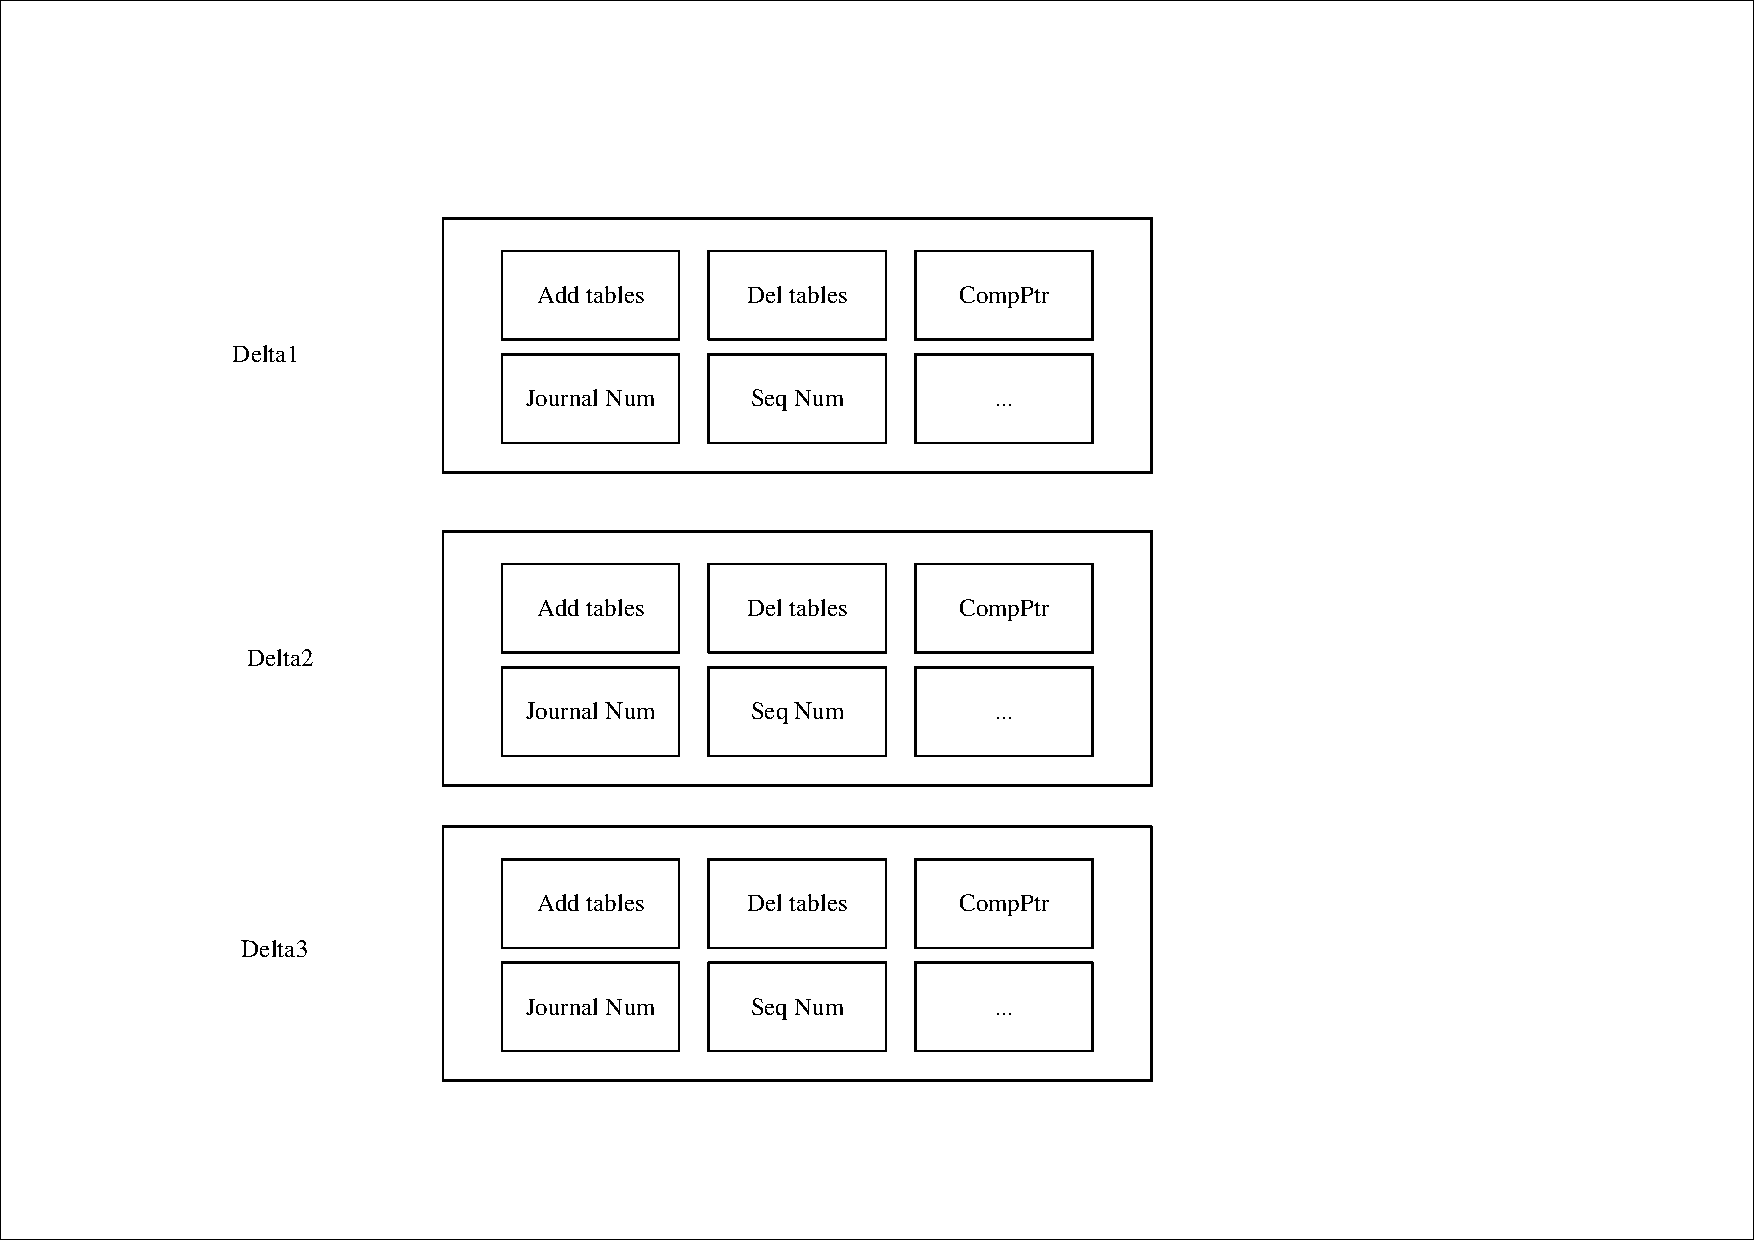
\includegraphics[width=0.80\textwidth]{pdf/manifest.pdf}
			\caption{版本信息记录数据结构}
			\label{radds_storage_manifest}
		\end{figure}

	
	
